\chapter{Présentation générale}
\section{Le groupe Thales}
\subsection{Historique du groupe}

Le groupe Thales actuel est la résultante d'une évolution complexe,  jalonnée par plusieurs fusions dont voici les principales :
\begin{center}
\includegraphics[height=10cm]{ressources/images/figures/timeline.png}
\end{center}

\begin{itemize}
    \item \textbf{1968 :} La branche électronique de Thomson-Brandt et la Compagnie Générale de Télégraphie fusionnent pour créer Thomson-CSF.
    \item \textbf{2000 :} Thomson-CSF fusionne avec Dassault Électronique et devient THALES.
    \item \textbf{2007 :} Les activités d'Alcatel-Lucent liées au transport, à l'espace ainsi qu'à la sécurité sont transférées vers Thales par le biais d'une fusion, qui mène aussi à la création de Thales Alenia Space.
    \item \textbf{2019 :} Après l'annonce en 2017 d'une offre de rachat de Gemalto, Thales a obtenu de la Commission européenne la validation de l'OPA. Cette dernière devrait avoir lieu au premier trimestre de cette année.
\end{itemize}

\subsection{Les domaines d'activités}

Thales est implantée dans 56 pays, et cela grâce à un large spectre de compétences, divisé en 5 secteurs d'activité qui sont :
\begin{itemize}
\item \textbf{La défense : }Thales est numéro 1 mondial dans la défense aérienne avancée et numéro 1 en Europe concernant l'électronique de défense. Les solutions conçues, déployées et maintenues par Thales concernent à la fois l'aérien, le terrestre, le spatial, le maritime ainsi que les communications radio, les systèmes interarmées et la cybernétique.
\item \textbf{La sécurité :} en 2011, deux sociétés du groupe Thales fusionnent pour former Thales Communications \& Security dont les domaines d'activité sont multiples : la sécurité urbaine, la protection d'infrastructures critiques telles que les aéroports, la sécurité des systèmes de communication ainsi que la cybersécurité.
\item \textbf{L'aéronautique :} Thales domine le domaine de la gestion du trafic aérien, deux tiers des avions possèdent à minima un équipement Thales que ce soit pour la navigation, la génération d'électricité, les solutions de divertissement ou encore les cockpits.
\item \textbf{L'aérospatiale :} la présence du groupe dans l'aérospatiale civile et militaire est assurée par Thales Alenia Space, un des leaders mondiaux dans la conception de satellites de communication. Cette société propose aussi des systèmes pour l'observation de la Terre, l'exploration, la navigation, le transport ainsi que les infrastructures spatiales (comme l'ISS).

\item \textbf{Les transports terrestres :} Thales élabore des solutions pour les grandes lignes ferroviaires, mais aussi pour des moyens de transports urbains comme le métro, le tramway ou encore le \gls{LRT}.
Le groupe développe des solutions innovantes, fondées sur des technologies de pointe comme le Système Européen de Contrôle des Trains (ETCS).
\end{itemize}


\subsection{Position du groupe sur la scène internationale}

Voici les chiffres réalisés par Thales en 2017 :

\begin{center}
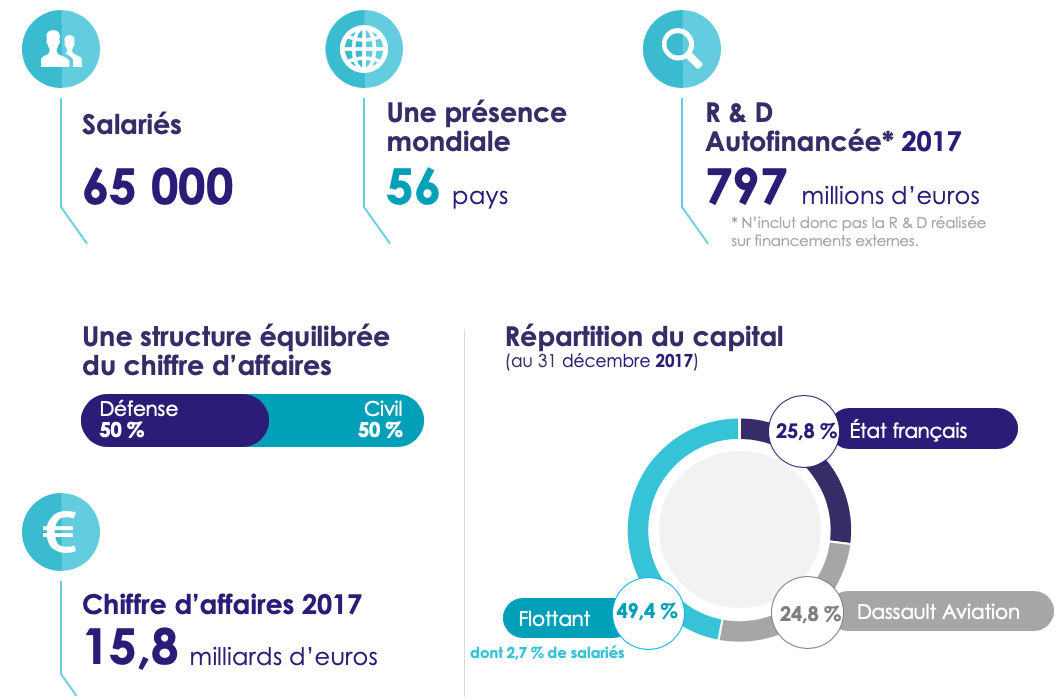
\includegraphics[height=8cm]{ressources/images/figures/Key.png}
\end{center}

En ce qui concerne la concurrence, Thales se positionne de la manière suivante :
\begin{itemize}
\item \textbf{Pour la signalisation ferroviaire :} même si Thales réalise un chiffre d'affaires annuel de 1,7 milliard d'euros, c'est son avance technologique dans le domaine des trains autonomes qui lui permettra de rivaliser avec le géant Siemens Alstom.
\item \textbf{Dans l'aéronautique :} les trois leaders français dans ce domaine sont Thales, Safran et Zodiac. Ainsi Thales se partage le marché des équipementiers civils, mais possède une position de poids dans le secteur de l'aéronautique militaire et plus particulièrement dans la défense, notamment grâce à la part importante de son capital dédiée à la partie Dassault Aviation du groupe.
\end{itemize}

\section{Le projet : Lusail LRT}
\subsection{Le Light Rail Transit} Le Transit Léger sur Rail ou Métro léger est une technologie de transport ferroviaire urbain. Sa vitesse moyenne et sa capacité de transport sont en général supérieures à celle d'un tramway, mais inférieures à celles d'un métro. Le \gls{LRT} adopte le fonctionnement d'un métro sur les tronçons souterrains et celui du tramway sur ceux en surface.
Du point de vue du fonctionnement, la différence principale entre le \gls{LRT} et le métro réside dans le fait que plusieurs lignes différentes peuvent circuler sur des tronçons de voies communs.
De nombreuses villes dans le monde ont déjà implanté un  \gls{LRT} dans leur réseau de transport en commun, telles que Hong Kong, Francfort, São Paulo, Ottawa ou encore Jérusalem.

\subsection{Le contexte du projet} Le projet se déroule dans la nouvelle ville de Lusail au Qatar située en périphérie de Doha, la capitale du pays. Cette ville, lorsqu'elle sera terminée, s'étendra sur 38 \begin{math} km^2 \end{math} et devrait accueillir 450 000 habitants. Elle tiendra une place centrale dans les activités culturelles, artistiques et sportives du pays avec par exemple le circuit international de Lusail, mais aussi le stade de football qui accueillera le match d'ouverture et la finale de la Coupe du Monde de football en 2022. Dans l'optique de désengorger le trafic routier ainsi que de préparer au mieux l'accueil de la Coupe du Monde, la ville de Doha se verra équipée prochainement de 3 lignes de métro et la ville de Lusail se verra équipée de 4 lignes de LRT. Le projet concerné par ce rapport est celui du LRT de Lusail. Ce dernier comportera 4 lignes, 37 stations (dont 2 reliées aux réseaux du métro de Doha), 28 rames pour une capacité totale de 50 000 voyageurs par jours.

\begin{center}
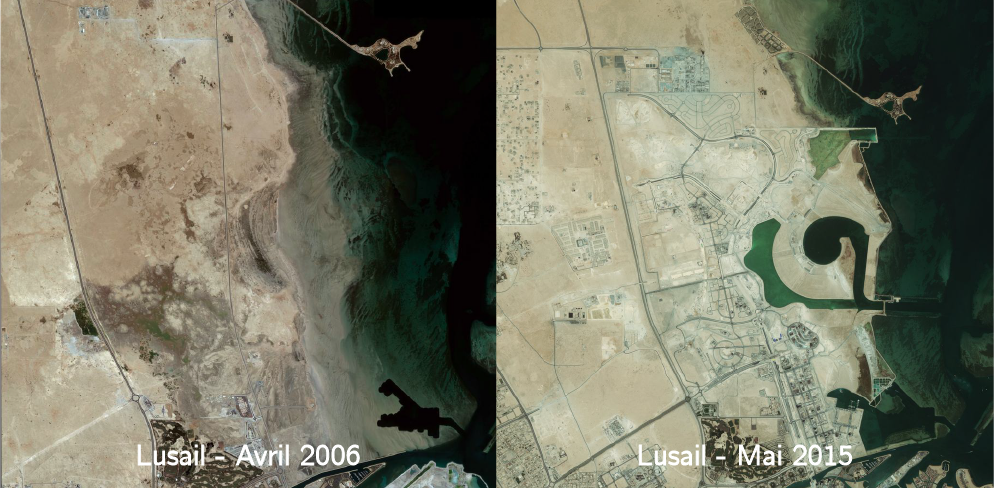
\includegraphics[height=8cm]{ressources/images/figures/Lusail.png}
\end{center}

\subsection{Les acteurs du projet}
De nombreuses entreprises sont engagées sur ce projet de transport, puisque celui-ci implique à la fois du génie civil, de l'ingénierie ferroviaire, des télécommunications ainsi que de la sécurité.
\begin{center}
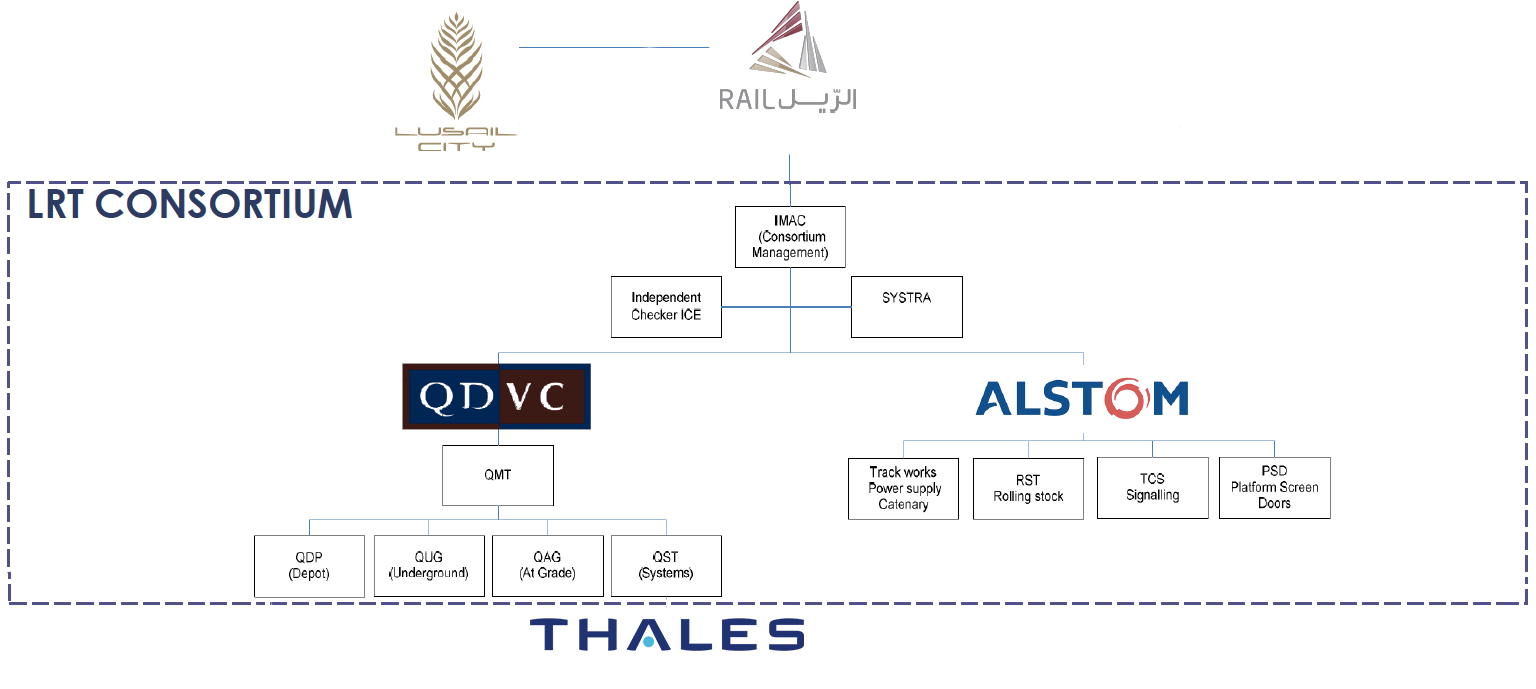
\includegraphics[height=8cm]{ressources/images/figures/Consortium.png}
\end{center}

\begin{itemize}
\item \textbf{Qatar Rail :} entreprise créée après le début de la phase de définition du projet, afin de superviser l'ensemble du réseau ferroviaire du pays. C'est l'employeur et donc le client direct du Consortium.
\item \textbf{IMAC :} entité de management du consortium, elle est composée à la fois d'employés de QDVC et d'Alstom, les deux entreprises principales du consortium et fait l'intermédiaire entre le consortium et le client.
\item \textbf{ICE :} entité de contrôle dont le rôle est assuré par la société SENER. Elle évolue de manière externe au consortium et donc indépendamment  de celui-ci afin de pouvoir certifier la conformité du système par rapport aux exigences du contrat au client Qatar Rails.
\item \textbf{SYSTRA :} entreprise réalisant pour l'IMAC des missions d'audit concernant le design. Elle est impliquée durant la phase de définition du projet en réalisant les différentes spécifications présentes dans le contrat, mais aussi durant la phase de réalisation afin d'orienter les stratégies d'opération.
\item \textbf{Alstom :} Alstom prend à charge toute la partie ferroviaire du projet : les rames (\gls{RST} : matériel roulant), la signalisation (\gls{TCS} : Système de contrôle du tramway), les portes palières (\gls{PSD} : portes palières) ou encore les caténaires.
\item \textbf{QDVC :} QDVC est une  filiale à 51\% de Qatari Diar et à 49\% de VINCI Construction Grands Projets. Elle prend à charge notamment le génie civil pour les bâtiments du dépôt, les bâtiments sous-terrains ainsi que les bâtiments à la surface, que ce soit des stations ou des bâtiments techniques. Cette entreprise sous-traite trois secteurs d'activité :
\begin{itemize}
\item \textbf{\gls{CCS} :} Systèmes de contrôle et de communication, cette partie est assurée par Thales.
\item \textbf{\gls{TVS} :} Système de Ventilation des Tunnels.
\item \textbf{\gls{ECS} :} Système de Contrôle Environnemental (température, humidité, etc.)
\end{itemize}
\item \textbf{RKH :} fruit de la fusion entre le consortium RATP Dev et Keolis (49\% ) et la société qatarie Hamad Group (51\%), RKH assurera l'exploitation et la maintenance du LRT de Lusail ainsi que du Métro de Doha.
\end{itemize}

\subsection{Place de Thales au sein du projet}

Sur ce projet, l'entreprise est positionnée en tant que sous-traitant de QDVC. Elle est en charge du design, de l'installation, des tests et de la mise en service des systèmes \gls{CCS}. Ces derniers sont organisés comme suit :

\begin{itemize}
\item \textbf{Télécommunications :} secteur d'activité clé de Thales, il représente une part importante du projet.
\begin{itemize}
\item \textbf{\gls{DTS} :} Système de Transmission Digitale, ensemble des différentes infrastructures réseau.
\item \textbf{Téléphonie :} Ce secteur englobe les téléphones présents dans les ascenseurs, dans les centres opérationnels ou encore la gestion de la téléphonie embarquée dans les rames lorsqu'elles circulent à la surface ou sous terre.
\item \textbf{\gls{TETRA} :} Système de radio mobile numérique destiné aux futurs opérateurs du système afin de leur assurer un moyen de communication fiable et sécurisé.
\item \textbf{BBRS :} Radio à large bande. %Préciser
\item \textbf{\gls{WA} :} Système permettant de proposer aux usagers du LRT de bénéficier d'un accès à Internet via un réseau WiFi.
\item \textbf{\gls{COMTV} :} Ensemble des écrans situés en station et à bord des rames ayant pour fonction de diffuser des annonces publicitaires aux usagers.
\item \textbf{\gls{UPS} :} Système d'alimentation sans interruption permettant de garantir la stabilité du réseau électrique, quelles que soient les interactions des différentes entités avec celui-ci.
\item \textbf{\gls{PIS}-\gls{PAS} :} Systèmes d'information visuelle et sonore destinés aux passagers, mais aussi plus généralement au public.
\end{itemize}
\item \textbf{Sécurité :} les trois systèmes de ce secteur sont implantés dans toutes les localisations du projet, c'est à dire les stations, les centres opérationnels, les bâtiments techniques et ceux du dépôt.
\begin{itemize}
\item \textbf{\gls{ACS-IDS} :} Système de Contrôle des Accès ainsi que de Détection des Intrusions.
\item \textbf{\gls{FDS} :} système de détection des incendies.
\item \textbf{\gls{CCTV} :} système de vidéosurveillance.
\end{itemize}
\item \textbf{Supervision :} ce secteur est primordial sur les projets ferroviaires urbains, car c'est lui qui permettra aux futurs opérateurs de gérer tout type situation.
\begin{itemize}
\item \textbf{\gls{SCADA} :} Système de Contrôle et d'Acquisition de Données, solution mise au point par Thales.
\item \textbf{\gls{MMS} :} Système de Management de la Maintenance.
\end{itemize}
\item \textbf{Billettique :} \gls{AFC} : Système de Collection Automatique des Billets
\end{itemize}


\section{Présentation de l'équipe T \& C}

Sur ce projet, Thales fonctionne avec des équipes offshore (Thales France, Thales Italy, Thales Portugal) et une équipe inshore sur place rattachée à Thales Gulf.
Ainsi, l'équipe projet est organisée comme ci-dessous :

\begin{center}
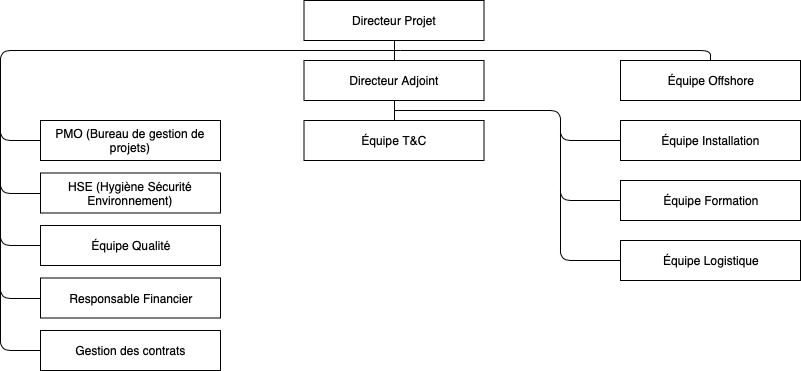
\includegraphics[height=8cm]{ressources/images/figures/OBS1.png}
\end{center}

En ce qui concerne l'équipe \gls{TC}, sa fonction principale est de tester et de mettre en service les systèmes et équipements \gls{CCS}.
Son organisation, qui compte environ une trentaine de personnes, est la suivante :

\begin{center}
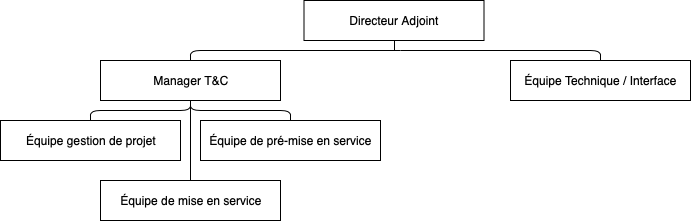
\includegraphics[height=5cm]{ressources/images/figures/OBS2.png}
\end{center}

QDVC est le client direct de Thales, mais agit aussi en tant qu'autorité de contrôle durant les différentes phases du projet, en suivant un cycle en V (cf. Annexe I). Concentrons-nous ici sur la phase de test : chaque test nécessite le témoignage et l'approbation de QDVC et de ICE, l'entité de contrôle indépendante.
Dans le but de pouvoir mettre en application ce système d'approbation, le client a fait le choix d'une base de données permettant l'édition dynamique (et donc la signature) de rapports de test au format PDF : \gls{SnagR}.
Afin d'assurer la communication et le contrôle des documents du référentiel projet, une base de données commune est utilisée : \gls{Mezzoteam}, mais Thales utilise aussi en parallèle une  base de données indépendante du client : \gls{e-TOL}.

Les méthodes utilisées à l'échelle macroscopique du projet sont des méthodes de gestion de projet dites "classiques" : on peut par exemple noter l'utilisation de Primavera, un outil permettant de générer un planning de type Gantt et proposant des outils d'estimation des coûts.
Au sein de l'équipe \gls{TC}, de nombreux outils sont utilisés (dont certains sont issus des \gls{methodesagiles}, mais nous reviendront sur ce point dans la prochaine partie) :
\begin{itemize}
\item \textbf{\gls{Git} :} Outil de gestion des versions et configurations logicielles.
\item \textbf{Doors :} logiciel de gestion des exigences.
\item \textbf{Giro :} logiciel de gestion des risques.
\item \textbf{Jira :} solution de gestion des incidents techniques.
\item \textbf{Palma :} logiciel de gestion des configurations.
\end{itemize}

Au sein de cette équipe, j'ai été encadré par mon maître de stage, Vincent ARGENTON et par Stéphane GLOAGUEN.

M.Argenton est le manager technique du projet du \gls{LRT} de Lusail, sur lequel il travaille depuis 4 ans et travaillait auparavant, toujours pour Thales, sur le projet du \gls{LRT} de Panama. Il est diplômé de l'école d'ingénieur ECE Paris et a également obtenu un master de Management de Projet International à l'ESCP Europe, à Madrid.

M.GLOAGUEN est le chef du département  \gls{TC} du projet, il occupait la même position sur le projet du Métro de Doha et travaille pour Thales depuis plus de 10 ans.
